% Template for PLoS
% Version 2.0 July 2014
%
% To compile to pdf, run:
% latex plos.template
% bibtex plos.template
% latex plos.template
% latex plos.template
% dvipdf plos.template
%
% % % % % % % % % % % % % % % % % % % % % %
%
% -- IMPORTANT NOTE
%
% Be advised that this is merely a template 
% designed to facilitate accurate translation of manuscript content 
% into our production files. 
%
% This template contains extensive comments intended 
% to minimize problems and delays during our production 
% process. Please follow the template 
% whenever possible.
%
% % % % % % % % % % % % % % % % % % % % % % % 
%
% Once your paper is accepted for publication and enters production, 
% PLEASE REMOVE ALL TRACKED CHANGES in this file and leave only
% the final text of your manuscript.
%
% DO NOT ADD EXTRA PACKAGES TO THIS TEMPLATE unless absolutely necessary.
% Packages included in this template are intentionally
% limited and basic in order to reduce the possibility
% of issues during our production process.
%
% % % % % % % % % % % % % % % % % % % % % % %
%
% -- FIGURES AND TABLES
%
% DO NOT INCLUDE GRAPHICS IN YOUR MANUSCRIPT
% - Figures should be uploaded separately from your manuscript file. 
% - Figures generated using LaTeX should be extracted and removed from the PDF before submission. 
% - Figures containing multiple panels/subfigures must be combined into one image file before submission.
% See http://www.plosone.org/static/figureGuidelines for PLOS figure guidelines.
%
% Tables should be cell-based and may not contain:
% - tabs/spacing/line breaks within cells to alter layout
% - vertically-merged cells (no tabular environments within tabular environments, do not use \multirow)
% - colors, shading, or graphic objects
% See http://www.plosone.org/static/figureGuidelines#tables for table guidelines.
%
% For sideways tables, use the {rotating} package and use \begin{sidewaystable} instead of \begin{table} in the appropriate section. PLOS guidelines do not accomodate sideways figures.
%
% % % % % % % % % % % % % % % % % % % % % % % %
%
% -- EQUATIONS, MATH SYMBOLS, SUBSCRIPTS, AND SUPERSCRIPTS
%
% IMPORTANT
% Below are a few tips to help format your equations and other special characters according to our specifications. For more tips to help reduce the possibility of formatting errors during conversion, please see our LaTeX guidelines at http://www.plosone.org/static/latexGuidelines
%
% Please be sure to include all portions of an equation in the math environment, and for any superscripts or subscripts also include the base number/text. For example, use $mathrm{mm}^2$ instead of mm$^2$ (do not use \textsuperscript command).
%
% DO NOT USE the \rm command to render mathmode characters in roman font, instead use $\mathrm{}$
% For bolding characters in mathmode, please use $\mathbf{}$ 
%
% Please add line breaks to long equations when possible in order to fit our 2-column layout. 
%
% For inline equations, please do not include punctuation within the math environment unless this is part of the equation.
%
% For spaces within the math environment please use the \; or \: commands, even within \text{} (do not use smaller spacing as this does not convert well).
%
%
% % % % % % % % % % % % % % % % % % % % % % % %



\documentclass[10pt]{article}

% amsmath package, useful for mathematical formulas
\usepackage{amsmath}
% amssymb package, useful for mathematical symbols
\usepackage{amssymb}

% cite package, to clean up citations in the main text. Do not remove.
\usepackage{cite}

\usepackage{hyperref}

% line numbers
\usepackage{lineno}

% ligatures disabled
\usepackage{microtype}
\DisableLigatures[f]{encoding = *, family = * }

% rotating package for sideways tables
%\usepackage{rotating}

% If you wish to include algorithms, please use one of the packages below. Also, please see the algorithm section of our LaTeX guidelines (http://www.plosone.org/static/latexGuidelines) for important information about required formatting.
%\usepackage{algorithmic}
%\usepackage{algorithmicx}

% Use doublespacing - comment out for single spacing
%\usepackage{setspace} 
%\doublespacing


% Text layout
\topmargin 0.0cm
\oddsidemargin 0.5cm
\evensidemargin 0.5cm
\textwidth 16cm 
\textheight 21cm

% Bold the 'Figure #' in the caption and separate it with a period
% Captions will be left justified
\usepackage[labelfont=bf,labelsep=period,justification=raggedright]{caption}

% Use the PLoS provided BiBTeX style
\bibliographystyle{plos2009}

% Remove brackets from numbering in List of References
\makeatletter
\renewcommand{\@biblabel}[1]{\quad#1.}
\makeatother


% Leave date blank
\date{}

\pagestyle{myheadings}

%% Include all macros below. Please limit the use of macros.

%% END MACROS SECTION


\begin{document}


% Title must be 150 characters or less
\begin{flushleft}
{\Large
\textbf{3D-Printable Micropipette}
}
% Insert Author names, affiliations and corresponding author email.
\\
Author1$^{1}$, 
Author2$^{2}$, 
Author3$^{3,\ast}$
\\
\bf{1} Author1 Dept/Program/Center, Institution Name, City, State, Country
\\
\bf{2} Author2 Dept/Program/Center, Institution Name, City, State, Country
\\
\bf{3} Author3 Dept/Program/Center, Institution Name, City, State, Country
\\
$\ast$ E-mail: Corresponding author@institute.edu
\end{flushleft}

% Please keep the abstract between 250 and 300 words
\section*{Abstract}

% Please keep the Author Summary between 150 and 200 words
% Use first person. PLOS ONE authors please skip this step. 
% Author Summary not valid for PLOS ONE submissions.   
\section*{Author Summary}



\section*{Introduction}

3D printing as a form of additive manufacturing has existed for decades althought the recent avalibilty of inexpensive desktop printers have made it feasible for consumers to design and print prototypes and even functional parts, and consumer goods.

The open source software movement and has spawned the additional areas of open source hardware, such as microcontroller boards (Arduino) as well as 3D printers themselves (RepRap).
Open source scientific instruments and laboratory equipment are being actively developed(openpcr.org, opensource lab book.)
3D-printable lab equipment is and an attractive idea because of the simplicity of downloading and printing a functional object for only the price of the raw material. 
In addition, end users can customize the equiment to their application. 
Some of the more clever printable parts that have emerged are ones that give a new function to a ubiquitous existing device.
For example a drill bit attachment was designed and printed to hold micro centrifuge tubes allowing a drill to be used for centrifuging samples. 
Although this may make a rather crude centrifuge it may be and adequate method that only costs pennies compared to commercially available centrifuges and could allow researchers in the developing world to better participate in science by reducing some finacial barriers of entry.

Printable micropipette designs can be found on 3D-part sharing websites (thiniverse).
While existing designs may require only pen springs, a gasket made from a balloon, and tape, none allow adjustment to know volumes nor have any been rigorously validated.
We present a pipette constructed from 3D printed parts that allows a 1 mL syringe to be actuated to an adjustable volume.
The scale marks on the syringe can be used to adjust the dispensed volume accurately without calibrating with a scale.



This is a test of the citations \cite{oppegard2010}.


% You may title this section "Methods" or "Models". 
% "Models" is not a valid title for PLoS ONE authors. However, PLoS ONE
% authors may use "Analysis" 
\section*{Materials and Methods}

% Results and Discussion can be combined.
\section*{Results}

% We only support three levels of headings, please do not create a heading level below \subsubsection.
\subsection*{Subsection 1}

\subsubsection*{SubSubsection 1.1}

\subsection*{Subsection 2}

\section*{Discussion}



% Do NOT remove this, even if you are not including acknowledgments.

\section*{Acknowledgments}


%\section*{References}

\bibliography{references}

% Either type in your references using
% \begin{thebibliography}{}
% \bibitem{}
% Text
% \end{thebibliography}
%
% OR
%
% Compile your BiBTeX database using our plos2009.bst
% style file and paste the contents of your .bbl file
% here.
% 

\section*{Figure Legends}
% This section is for figure legends only, do not include3
% graphics in your manuscript file.
%
%\begin{figure}
%\includegraphics[scale=1]{file.png} % take image out for final manuscript
%\caption{
%{\bf Bold the first sentence.}  Rest of figure caption.  
%}
%\label{Figure_label}
%\end{figure}

\begin{figure}
%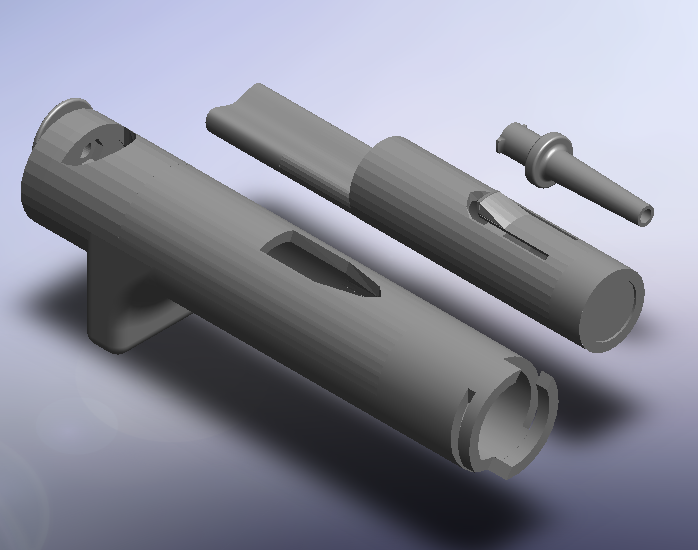
\includegraphics[scale=0.4]{figure-images/rendering-assembly4.png} % take image out for final manuscript
\caption{
{\bf CAD rendering of printable parts.}  Three parts are printed: the body, plunger shaft, and luer-lock adapter for pipette tips.
}
\label{CAD-render-figure}
\end{figure}

\begin{figure}
%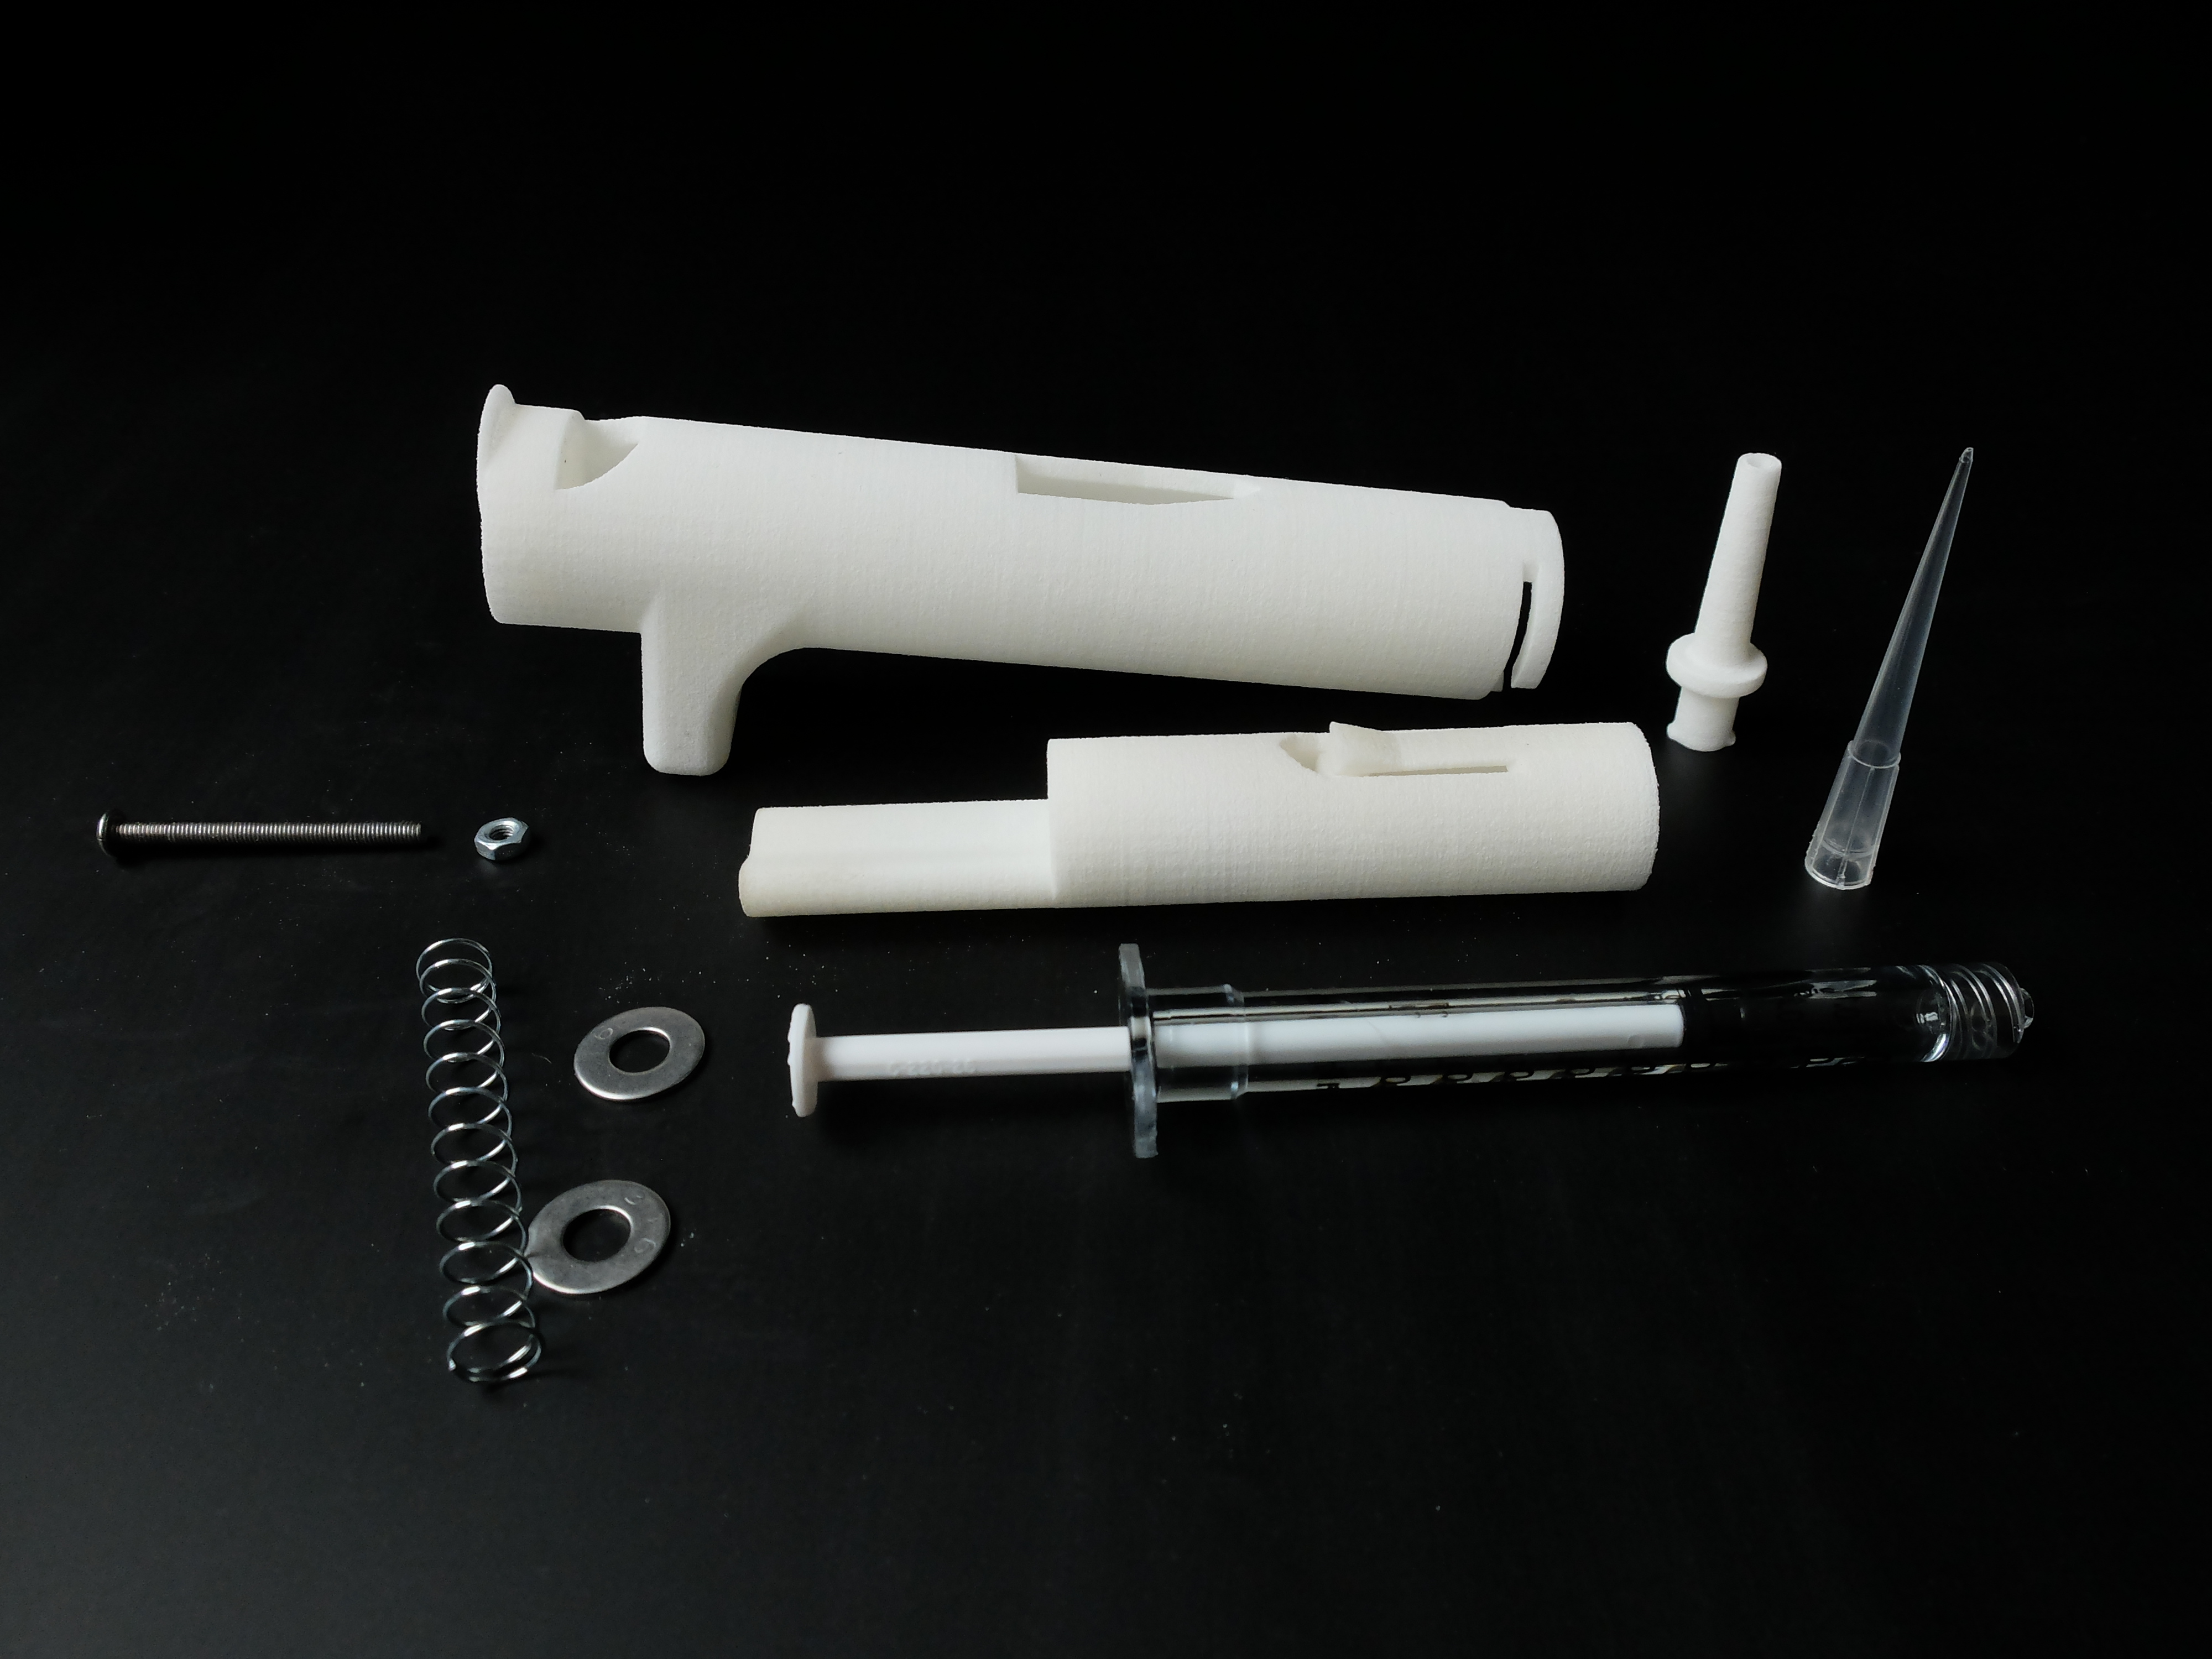
\includegraphics[scale=0.04]{figure-images/pipette-disassembled.JPG} % take image out for final manuscript
%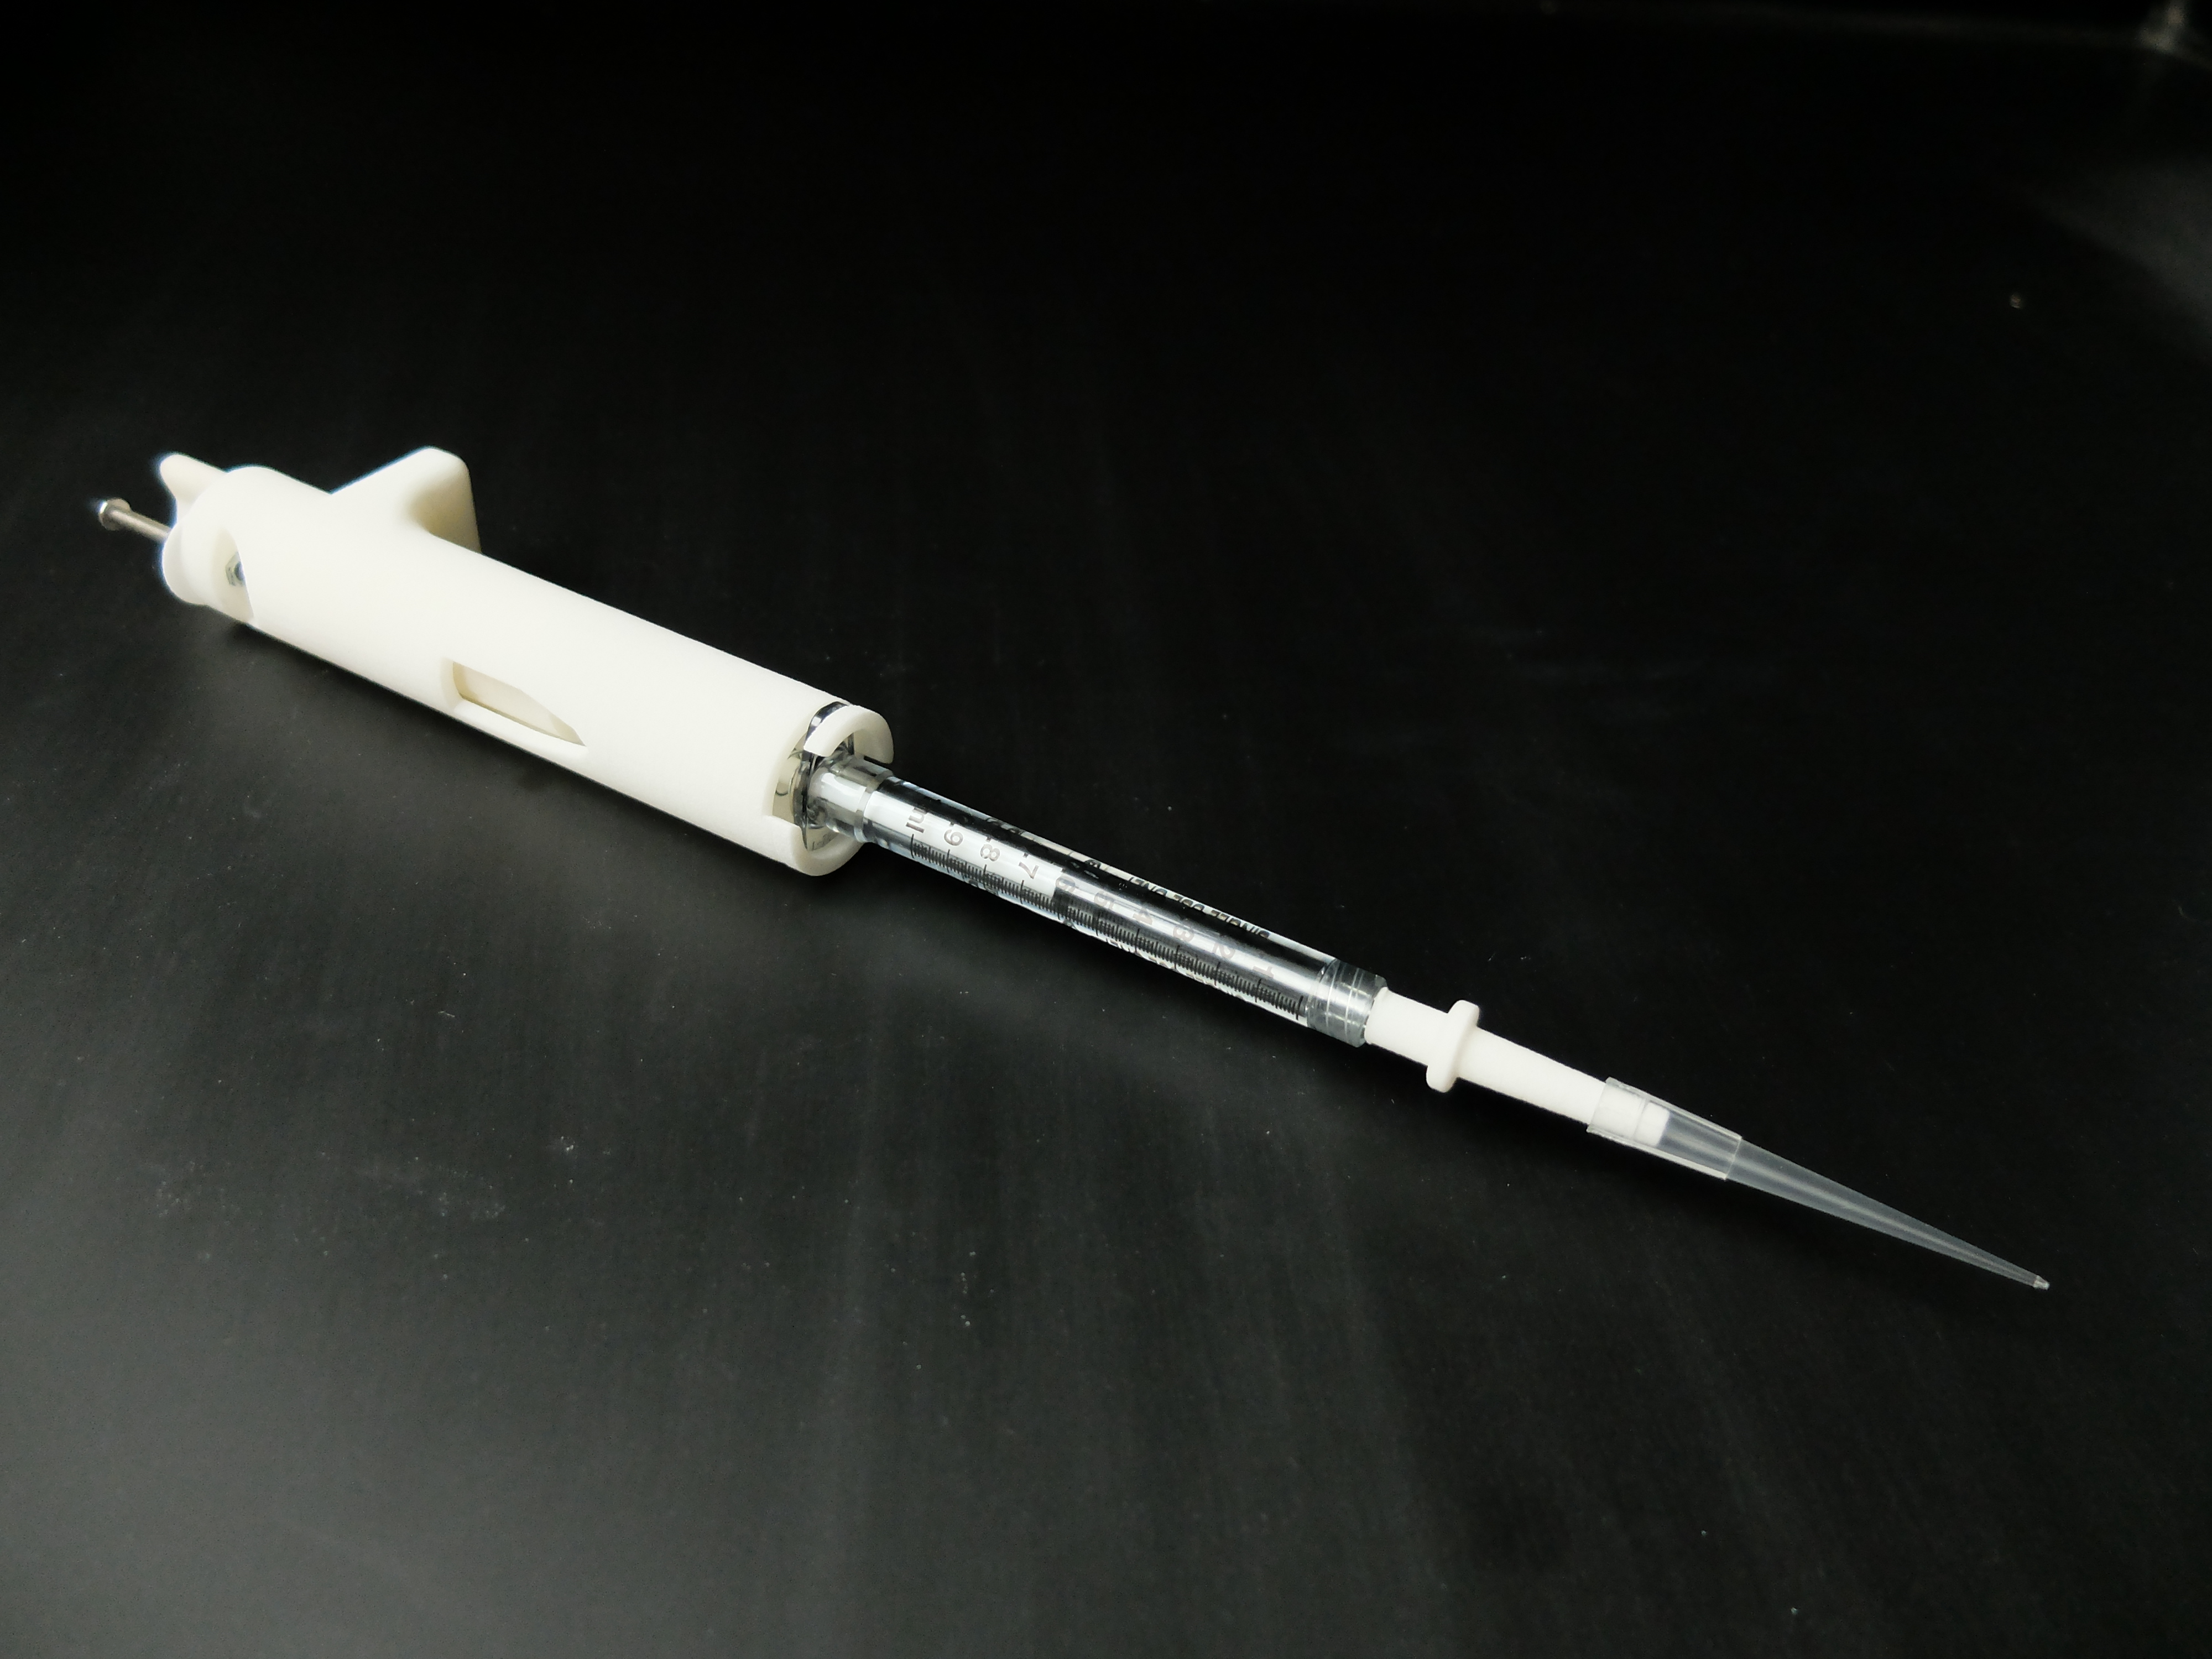
\includegraphics[scale=0.04]{figure-images/pipette-assembled.JPG} % take image out for final manuscript
\caption{
{\bf Photos of pipette.}  The pipette is composed of three printed parts, a 1 mL syringe and some additional hardware.  
}
\label{photo-parts-figure}
\end{figure}

%\begin{figure}
%\includegraphics[scale=1]{file.png} % take image out for final manuscript
%\caption{
%{\bf Bold the first sentence.}  Rest of figure caption.  
%}
%\label{Figure_label}
%\end{figure}


\section*{Tables}
% 
% See introductory notes if you wish to include sideways tables.
%
% NOTE: Please look over our table guidelines at http://www.plosone.org/static/figureGuidelines#tables to make sure that your tables meet our requirements. Certain types of spacing, cell merging, and other formatting tricks may have unintended results and will be returned for revision.
%
%\begin{table}[!ht]
%\caption{
%\bf{Table title}}
%\begin{tabular}{|c|c|c|}
%table information
%\end{tabular}
%\begin{flushleft}Table caption
%\end{flushleft}
%\label{tab:label}
% \end{table}

\begin{table}[!ht]
\caption{
\bf{Comparision of Accuracy and Precision}}
\begin{tabular}{|c|c|c|c|}
\hline
    Target Volume & 20 $\mu$L & 50 $\mu$L & 200 $\mu$L  \\
    \hline
    Printed Pipette & 196.4 $\pm$ 2.2 & 53.5 $\pm$ 1.8 & 19.5 $\pm$ 0.6 \\
    Commercial Pipette & 204.5 $\pm$ 2.9 & 49.9 $\pm$ 0.1 & 19.9 $\pm$ 0.2 \\
    \hline
\end{tabular}
\begin{flushleft} Average measured volume by weight and standard deviation.
\end{flushleft}
\label{tab:comp}
 \end{table}

\section*{Supporting Information Legends}
%
% Please enter your Supporting Information captions below in the following format:
%\item{\bf Figure SX. Enter mandatory title here.} Enter optional descriptive information here.
% 
%\begin{description}
%\item {\bf}
%\item {\bf}
%\end{description}

\end{document}

